                                % Created 2020-11-20 Fri 00:27
                                % Intended LaTeX compiler: pdflatex
\documentclass[11pt]{article}
\usepackage[utf8]{inputenc}
\usepackage[T1]{fontenc}
\usepackage{graphicx}
\usepackage{grffile}
\usepackage{longtable}
\usepackage{wrapfig}
\usepackage{rotating}
\usepackage[normalem]{ulem}
\usepackage{amsmath}
\usepackage{textcomp}
\usepackage{amssymb}
\usepackage{capt-of}
\usepackage{hyperref}
\author{Massimiliano Falzari(s3459101),  Philip Gast (s3149951)}
\date{\today}
\title{Assignment 1 Data analytics \& communication}
\hypersetup{
  pdfauthor={Massimiliano Falzari(s3459101),  Philip Gast (s3149951)},
  pdftitle={Assignment 1 Data analytics \& communication},
  pdfkeywords={},
  pdfsubject={},
  pdfcreator={Emacs 27.1 (Org mode 9.3)},
  pdflang={English}}
\begin{document}

\maketitle
\tableofcontents


\section{Finding the gaps in Bachelor projects}
\label{sec:org11e7944}
\subsection{Summary}
\label{sec:org1050e6c}
\url{http://fse.studenttheses.ub.rug.nl/id/eprint/21026}
This bachelor project is mainly focused on the performance of some
particular reinforcement learning techniques.
It focuses his attention on the game of soccer for different
reasons.  It starts giving a background of what was done in the
past and then it explains which techniques they are going to use
and test. They make different player which uses different
underlying reinforcement learning algorithms. The reference player
uses a multilayer perceptron(MLP) with a Q-learning
algorithm. Their main focus was on the type of perception given to
the agent/player. Therefore they had another player which instead
of a MLP uses a vision grid to process the perception of the agent.
Lastly, they also study how the activation function of the MLP
influence the results.
Finally, for every combination of field,team size and
agent they conduct an experiment. The final result shows that the
vision grid player performed significantly better then the MLP
player. However, they also noticed that the activation function of
the MLP can change a lot the performance of the agent.


\subsection{Flaws}
\label{sec:org56bed90}
The first part is quite good, there is no evident flaw in it. They describe all the various techniques accurately.
Probably the biggest flaw is that in the result section there are no statistical analyses.
However, apart from the result section, all the other section are clear and flawless.
\subsection{Improvements}
\label{sec:org8654ff3}
The possible improvements are :
\begin{itemize}
\item Statistical analyses
  Probably with some statistical analyses the project will result in more credible and also it probably allows to a different conclusion than the one presented.
\item More techniques
  They test just two techniques for the reinforcement learning part (e-greedy and softmax),
  maybe could be useful to see how other techniques behave with the vision grid technique.
\end{itemize}
\section{Making sure a planned Bachelor project is replicable and reproducible}
\label{sec:orgc2efad9}
\subsection{Reproducibility \& Replicability}
\label{sec:org4222b8f}
A potential Bachelor project would be to compare machine learning
techniques in face recognition. This project will look at different
machine learning techniques and use these techniques to use a system
to recognize faces. The accuracy of the machine learning technique in
recognizing faces will be compared.



Reproducibility describes how easy it is to repeat the study exactly
as it was done before. Replicability describes whether the results of
the study are the same when it is repeated.


In order to make this project reproducible I would have to make sure
that the sample size to compare the machine learning techniques is
large enough. I would also have to make sure that I change the context
in which the faces have to be recognized, so different lighting
scenery etc. The results for each face recognition task has to be
recorded and put in the research. The sample that is used in this
research is static since they are pictures of faces. If these pictures
are also included in the research it would increase the
reproducibility of the research.


In order to make this project replicable a large amount of pictures of
faces should be used. The research uses a static sample that can be
used by anyone who has access to it, enabling this sample for everyone
improves the replicability of this research. Since this research uses
machine learning it is important to note at how many samples a certain
system has seen, this is important for the end result. The person that
is repeating the study has to know how much input a system has had in
order to achieve the end result. If this is unknown the research would
not be replicable.


\section{Getting familiar with the tidyverse}
\label{sec:orgef73762}
\subsection{Data Manipulation}
\label{sec:orgdaa9a80}
\begin{itemize}
\item Transforming the duration of the delay from minutes into hours
\begin{verbatim}
  library(tidyverse)
  library(ggplot2)
  dat <- read.csv('disruptions-2019-Q4.csv')
  dat.tib <- as_tibble(dat)


  hours <- dat.tib %>%
  mutate(duration_hours= duration_minutes / 60)
\end{verbatim}
\item Counting the number of delays for the different groups of causes of delays
\begin{verbatim}
  count(hours,cause_group)
\end{verbatim}
\item Creating a dataframe which only consists of delays that have a known cause, and that are less than 20hours in duration.Make sure you combine both of these operations in one line of code.

\begin{verbatim}
  known_causes <-
  filter(hours,cause_group != "" &
  cause_group != "unknown" &
  duration_hours < 20)
\end{verbatim}
\item Using the data from c., creating an histogram using ggplot of the durations of delays that are found inthis sample. Make sure your plot has proper axes, focuses on the relevant part of the data, and is easy to read
\begin{verbatim}
  ggplot(known_causes,aes(duration_hours))+
  geom_histogram(binwidth = 1) + theme(text = element_text(size = 20))
\end{verbatim}
\begin{center}
  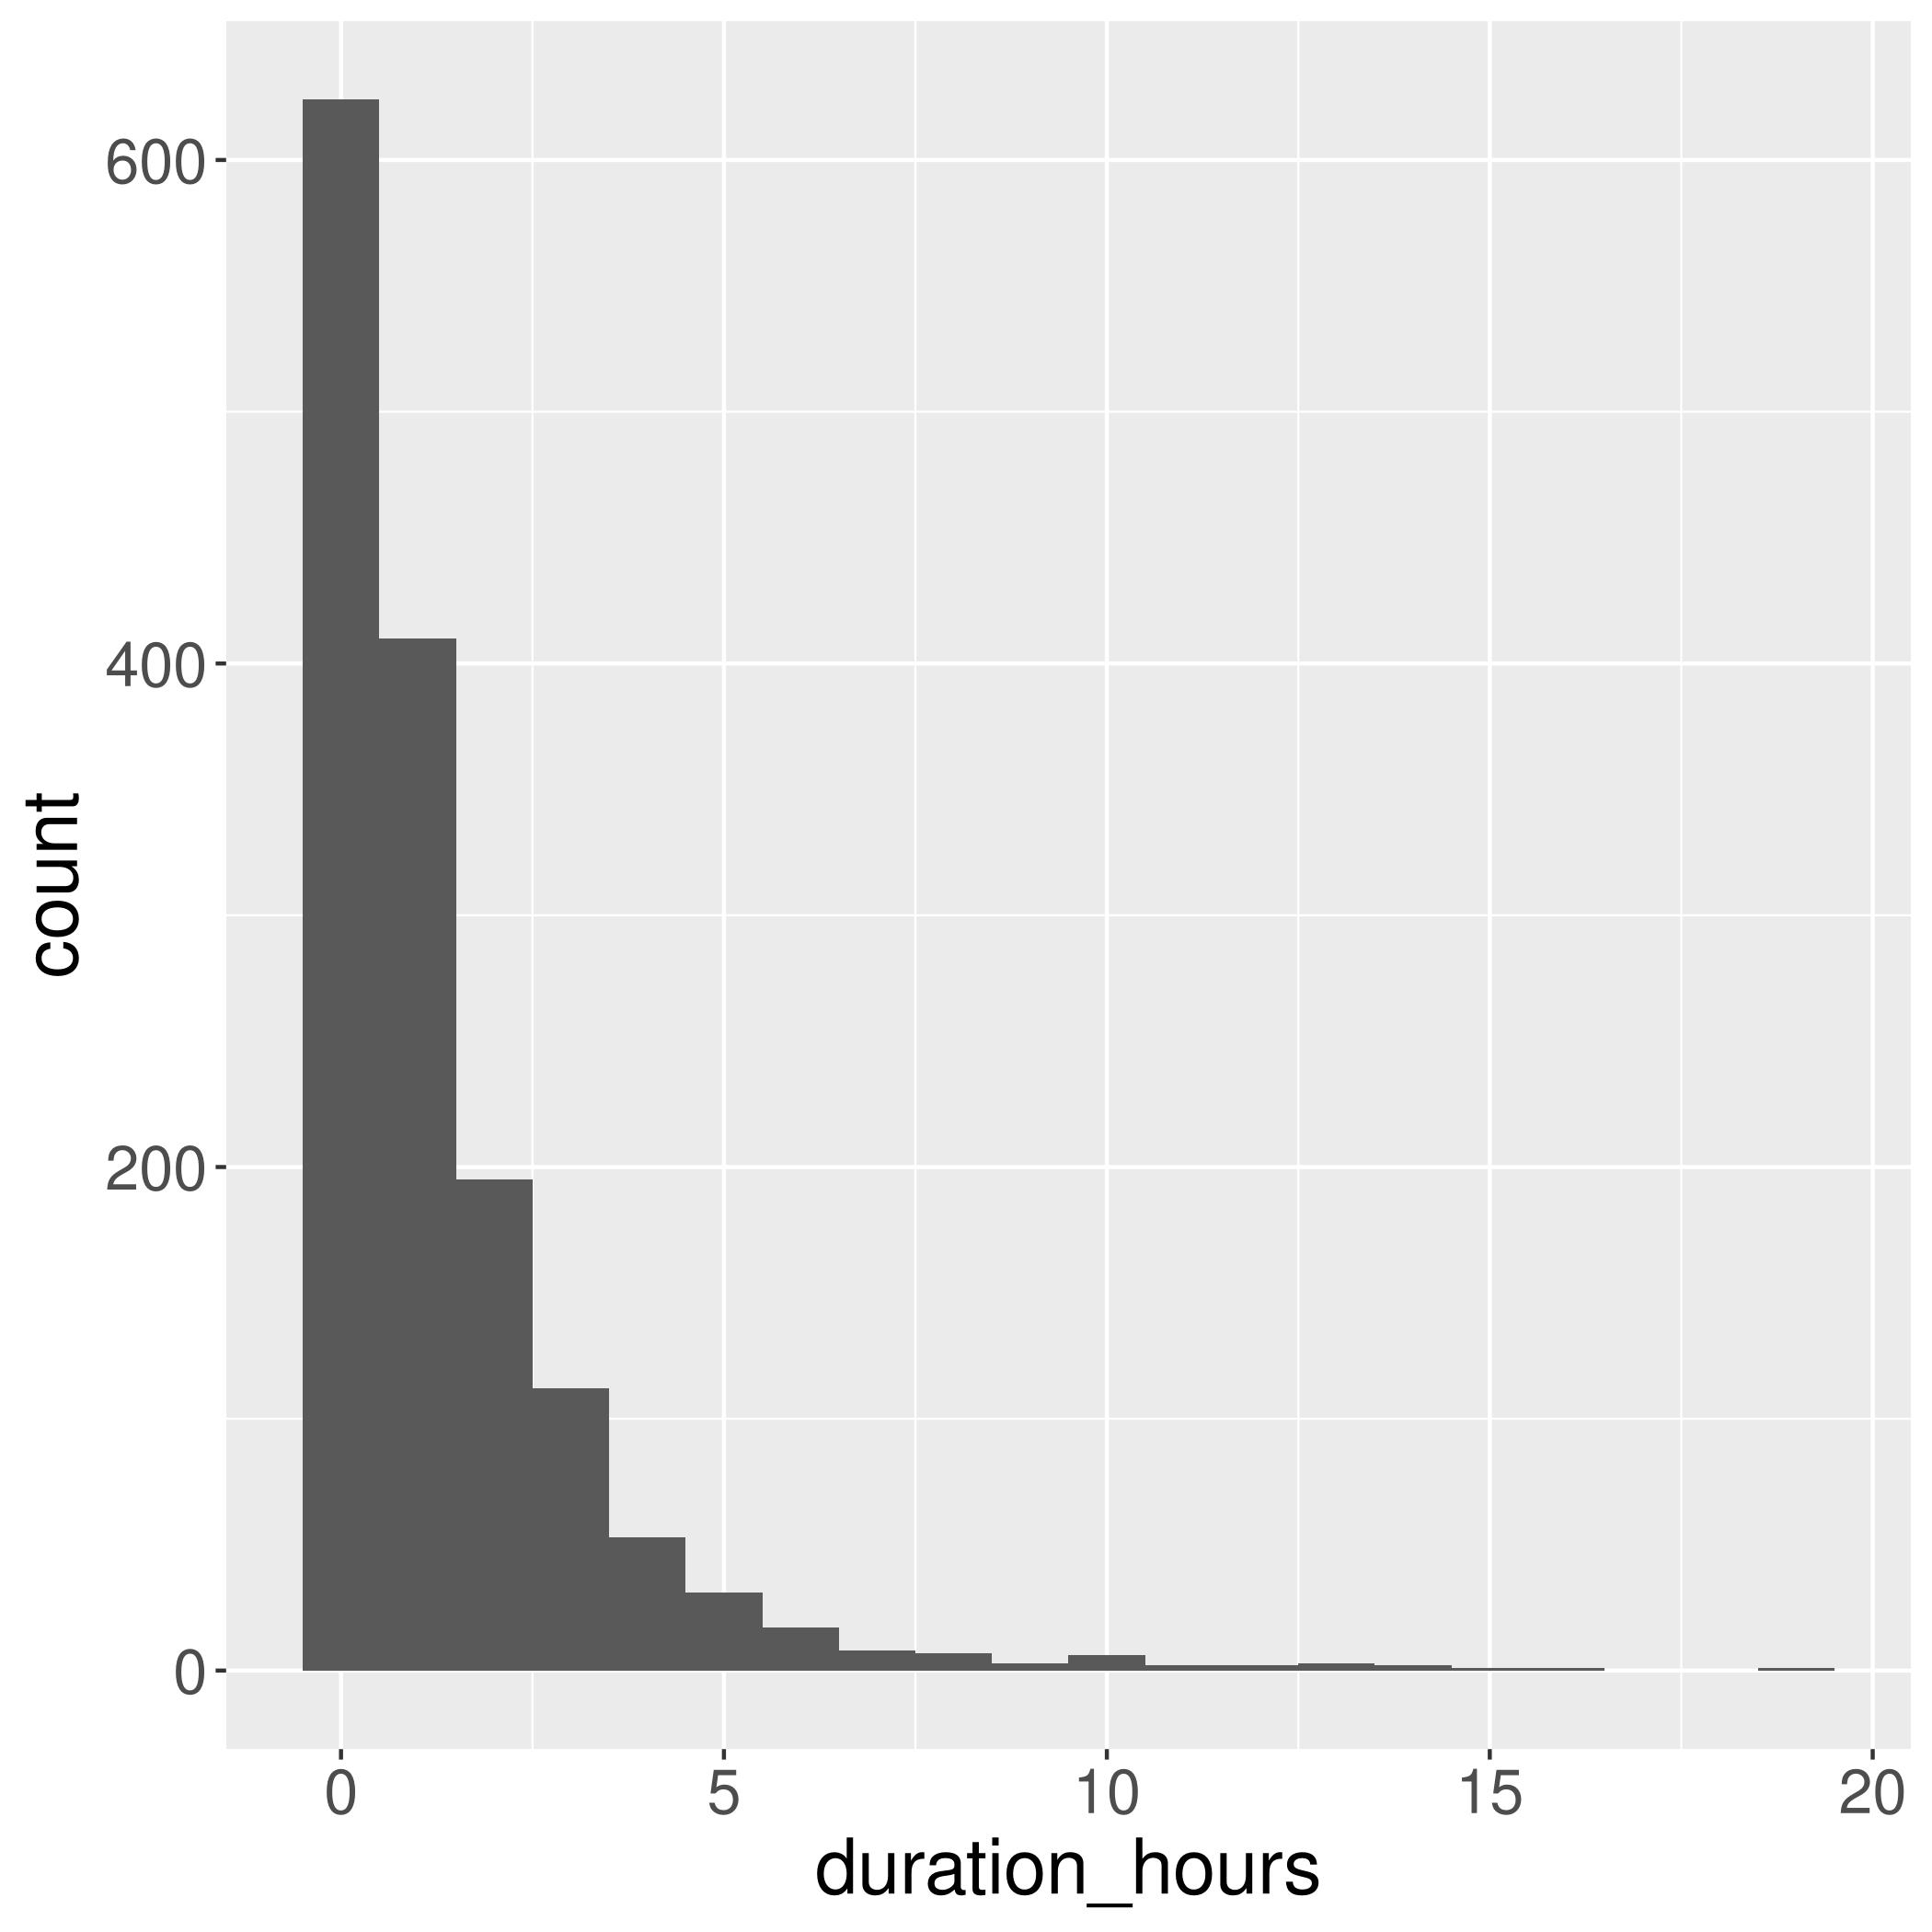
\includegraphics[width=.9\linewidth]{known_causes.jpg}
\end{center}
\end{itemize}
\subsection{Summarizing data}
\label{sec:org197e537}
\begin{verbatim}
  avg_delay_causes <- group_by(known_causes,cause_group) %>%
  summarize(avg=mean(duration_hours))

  ggplot(avg_delay_causes,aes(cause_group,avg)) +
  geom_bar(stat="identity")+ theme(text = element_text(size = 8.5))
\end{verbatim}

\begin{center}
  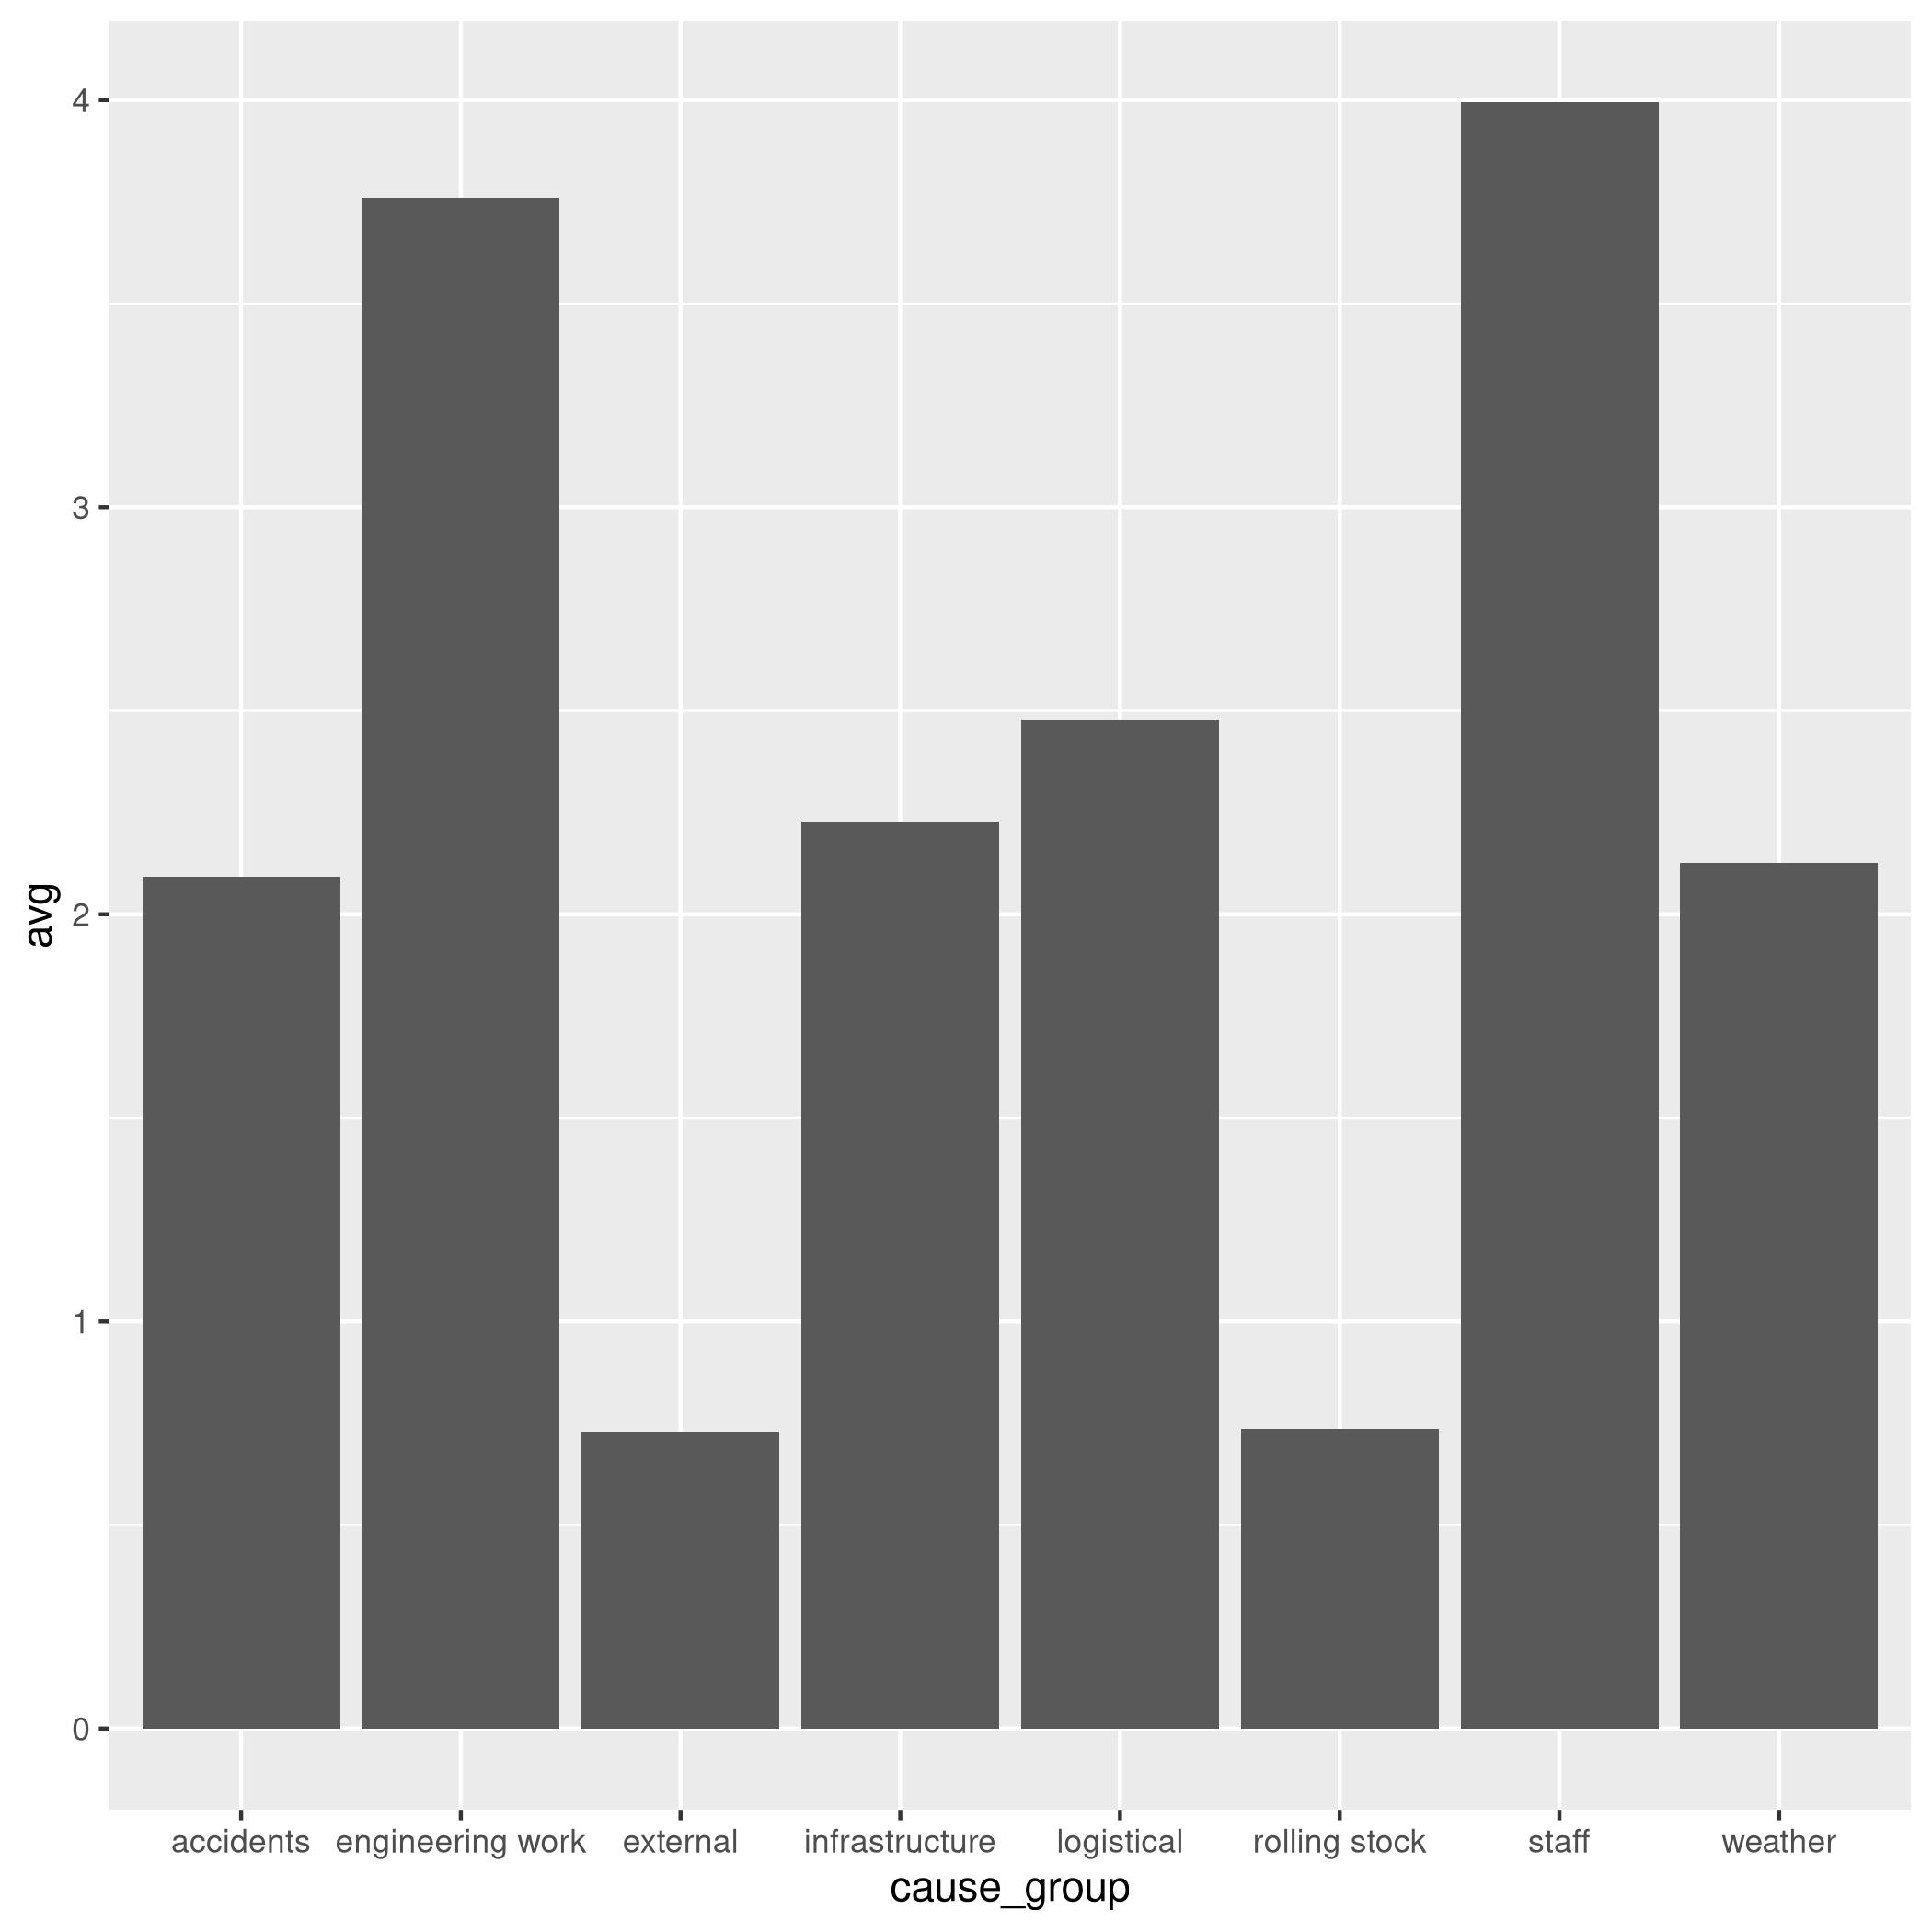
\includegraphics[width=.9\linewidth]{avg_delay_causes.jpg}
\end{center}


From this graph we can notice that the longer delays are usually
due to "staff" or engineering work causes. On the other hand
shorter delays are usually due to external or rolling stock causes.

\subsection{Spreading and gathering data}
\label{sec:orga0377ff}

In theory, the code below should gather the 1999 and 2000 columns into 2 new columns:
year and cases. In the column year the key of these columns will be insert (e.g. 1999 or 2000),
in the other column, cases,the value of associated with the key will be insert (e.g. 745 , 2666\ldots{}).
The firsts arguments to gather are similar to the select arguments.
The key argument is the name of the variable which values, form the column key.
The value argument is the associated value for that column

\begin{verbatim}
  table4a %>%
  gather(1999,2000,key = "year", value = "cases")
\end{verbatim}
It fails simply because there are missing backticks arround the numbers (they are non-syntactic names).
In the tibble they are store as character instead of numbers and therefore this line will always fails.
\begin{verbatim}

  people <- tribble(
  ~name,~key,~value,
  "Phillip Woods", "age", 45,
  "Phillip Woods","height",186,
  "Phillip Woods","age", 50,
  "Jessica Cordero","age",37,
  "Jessica Cordero","height",156)
  people %>%
  spread(key,value)
\end{verbatim}

the operation spread fails on the people tibble because there is not a unique combination
of keys which identify uniquely each row
\subsection{Separating \& uniting}
\label{sec:org4d5fa50}
\begin{itemize}
\item "extra: If ‘sep’ is a character vector, this controls what
  happens when there are too many pieces. There are three valid
  options:
  \begin{itemize}
  \item "warn" (the default): emit a warning and drop extra  values.
  \item "drop": drop any extra values without a warning.
  \item "merge": only splits at most ‘length(into)’ times " (from the R
    help function)
  \end{itemize}

\item "fill: If ‘sep’ is a character vector, this controls what
  happens when there are not enough pieces. There are three valid
  options:
  \begin{itemize}
  \item "warn" (the default): emit a warning and fill from the right
  \item "right": fill with missing values on the right
  \item "left": fill with missing values on the left " (from the R
    help function)
  \end{itemize}
\end{itemize}


\begin{verbatim}
  tibble(x =c("a,b,c", "d,e,f,g", "h,i,j")) %>%
  separate(x,c("one", "two", "three"),extra="merge")
  # Result :
  # A tibble: 3 x 3
  #  one   two   three
  #  <chr> <chr> <chr>
  # 1 a     b     c
  # 2 d     e     f,g
  # 3 h     i     j

  tibble(x =c("a,b,c", "d,e", "f,g,i")) %>%
  separate(x,c("one", "two", "three"),fill="left")

  # Result:
  # A tibble: 3 x 3
  #  one   two   three
  #  <chr> <chr> <chr>
  # 1 a     b     c
  # 2 NA    d     e
  # 3 f     g     i
\end{verbatim}
\end{document}
